\documentclass{article}
\usepackage[utf8]{inputenc}
\usepackage[margin =1in,includefoot]{geometry}
\usepackage{indentfirst}
\usepackage{graphicx}
\usepackage{float}
\usepackage{caption}
\usepackage{subcaption}
\usepackage[colorlinks=true, linkcolor = blue, urlcolor = cyan]{hyperref}

\title{Assignment 0 - COL380}
\author{Aayush Goyal}
\date{October 2021}

\begin{document}

\maketitle

\tableofcontents

% \newpage

\section{Introduction}
In this assignment, we will use perf tool to analyze the performance of a program. We will also use the perf tool to analyze the performance of a program after doing different optimizations like removing false sharing, removing memory leaks, etc. We will compare the performance of the program before and after the optimizations based on different metrics like cache misses, branch misses, etc.

\section{Setting up and Running Perf}
I used css1 to check the runtime of the code. For the report files I have used perf on my local machine since it was not working on the css machine. Same issue was faced by a lot of students.

\subsection{Perf stat}
I have varied the number of threads as 1, 4, 8, \dots, 32 keeping the number of iterations fixed as 3. There is a significant decrease till we use 16 threads, because this is the maximum number of threads we can run in parallel on the css machine. After this point the run-time does not decrease significantly because they are not actually running on different threads. They are just running like concurrent processes after that and this doesn't reduce the run-time significantly. However using more and more threads adds the overhead of thread management and context switching. Hence we can observe an increase in the number of cycles required to run the program. So it is best to use not more than 16 threads.
\begin{figure}[H]
\centering
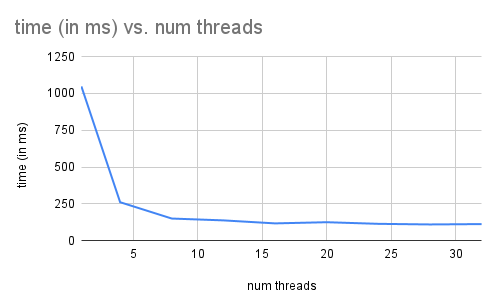
\includegraphics[width=0.7\textwidth]{images/time_threads.png}
\end{figure}

\begin{figure}[H]
\centering
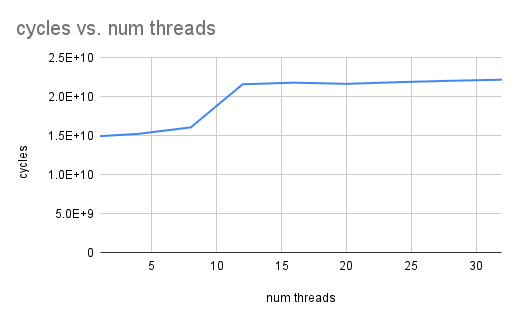
\includegraphics[width=0.7\textwidth]{images/cycles_threads.png}
\end{figure}

\subsection{Perf Record}
\subsubsection{}
After running the \texttt{perf record make run} command, we get the \texttt{perf.data} file. I have saved it with separate name as mentioned in the assignment.

\subsubsection{}
We obtained the perf data after running the previous command. This is not readable by humans and hence we need to use perf to read it. It is done using the following command \texttt{perf report -i <filename>}

\subsubsection{}
The instruction marked in red takes the most amount of time. perf marks the instructions which take the most amount of time (or whatever metric we are using). \texttt{jg 93} instructions takes the most time.

\subsubsection{}
Yes this can be easily done by adding \texttt{-g} flag in the CFLAGS during the compilation in the Makefile. Now after this we can see the annotated assembly code along with which source code it points to.

\begin{figure}[H]
\centering
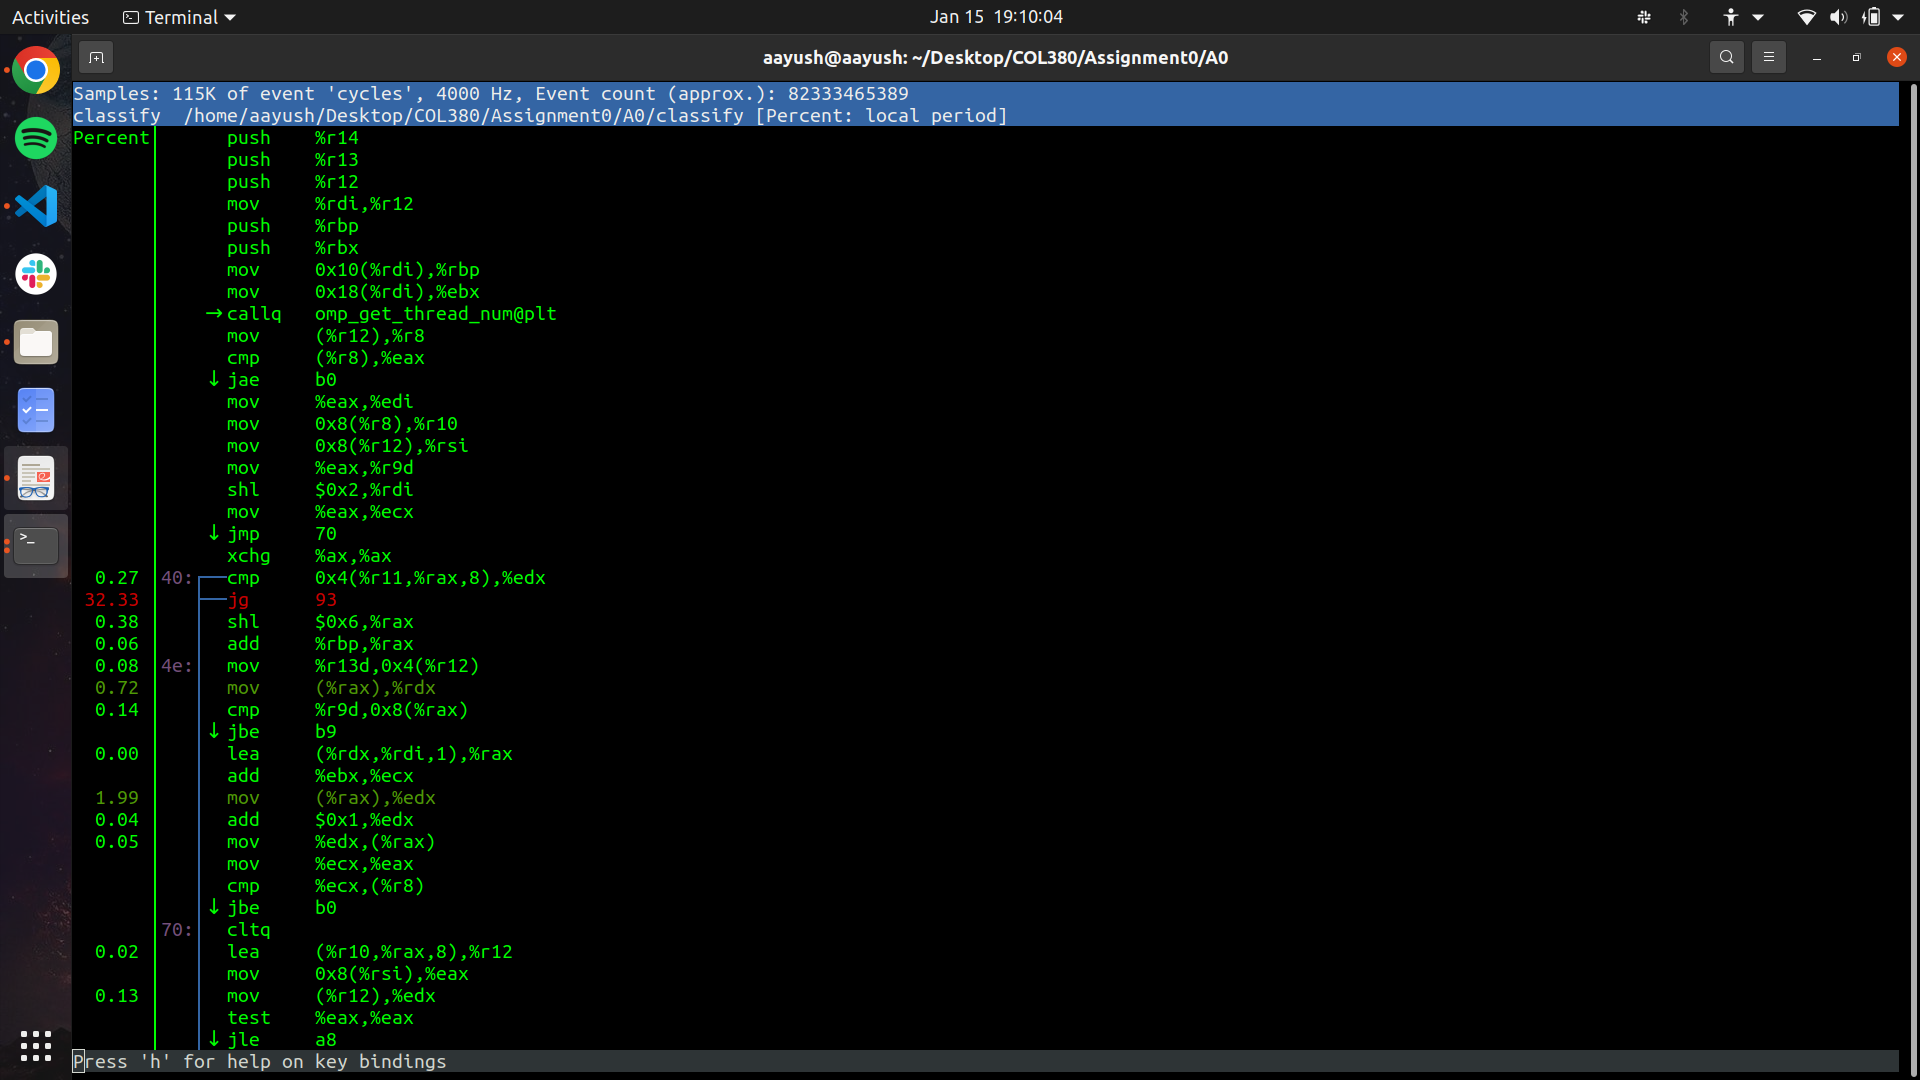
\includegraphics[width=1\textwidth]{images/2_3.1.png}
\end{figure}



\begin{figure}[H]
    \centering
    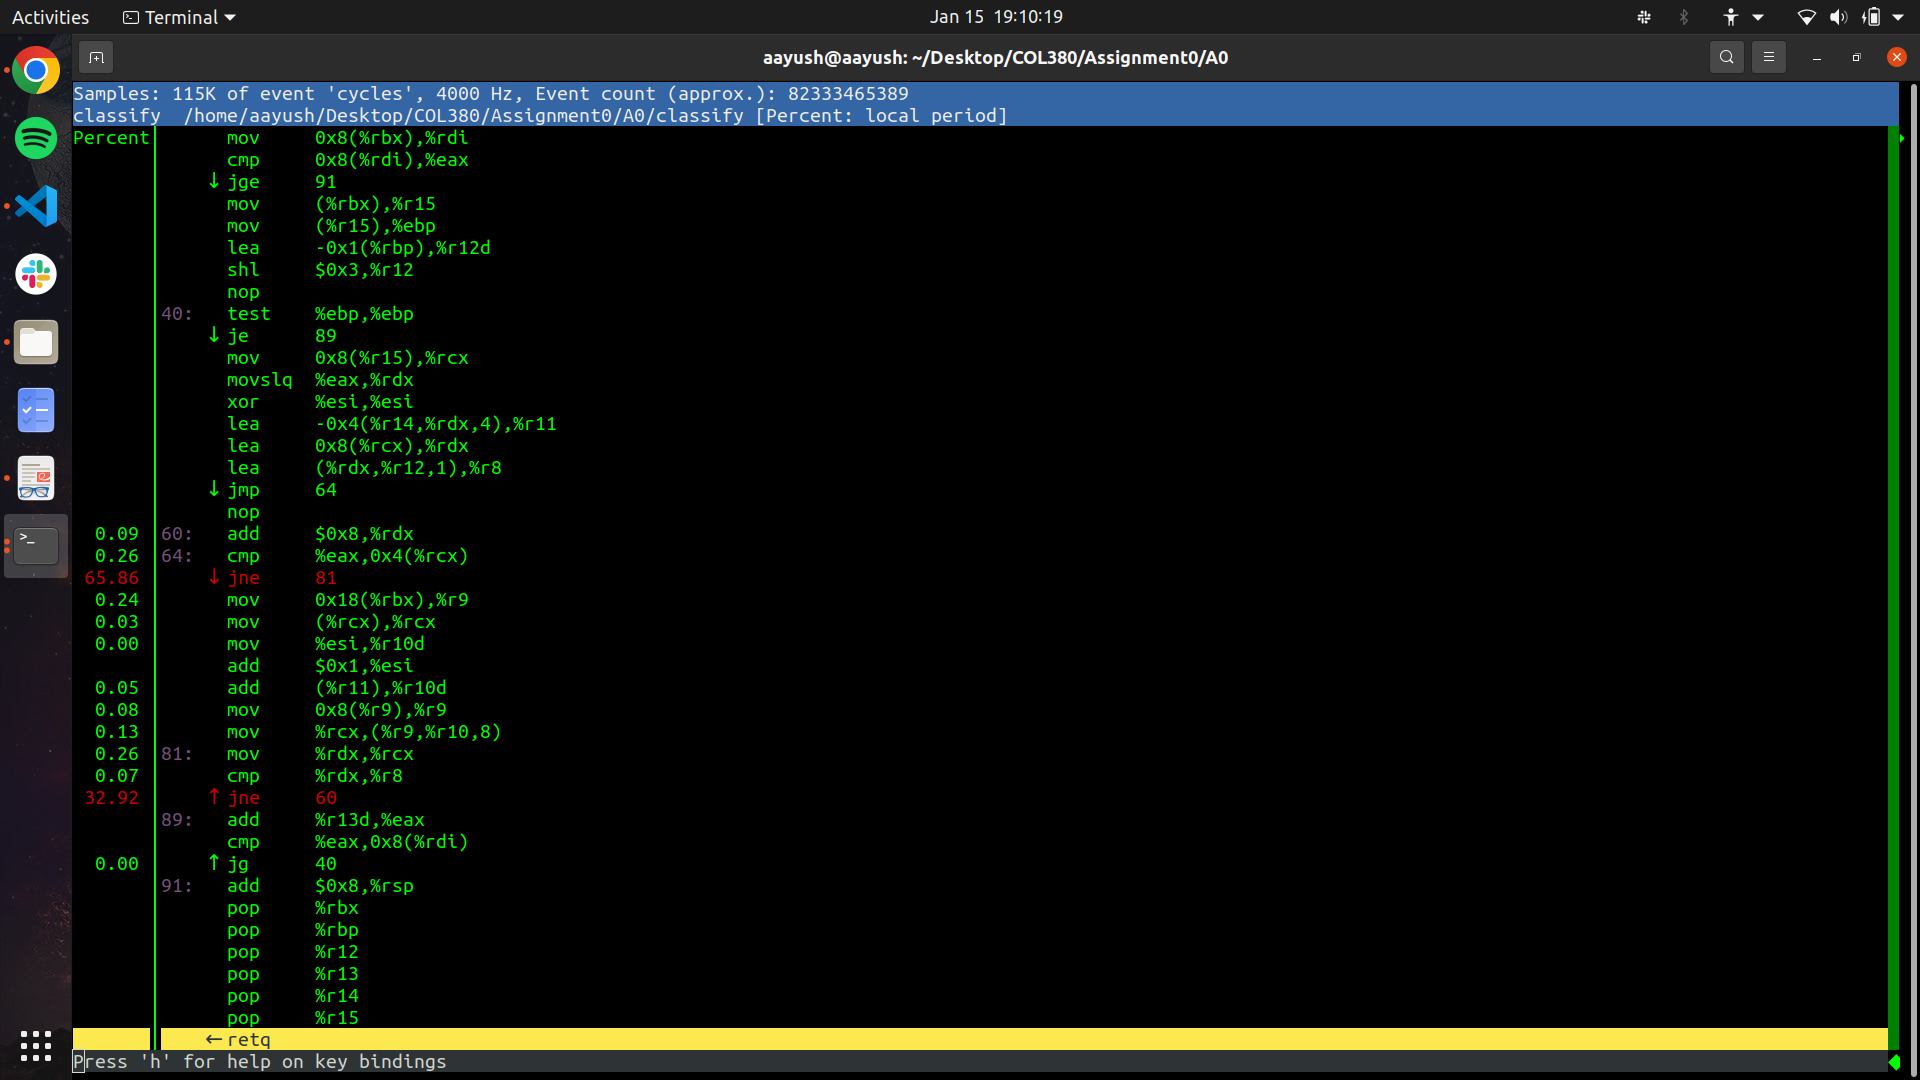
\includegraphics[width=1\textwidth]{images/2_3.2.png}
    \end{figure}

\subsubsection{}
Make the following change: \texttt{CFLAGS=-std=c++11 -O2 -g} and we can see the source code along with the assembly instructions.

\begin{figure}[H]
\centering
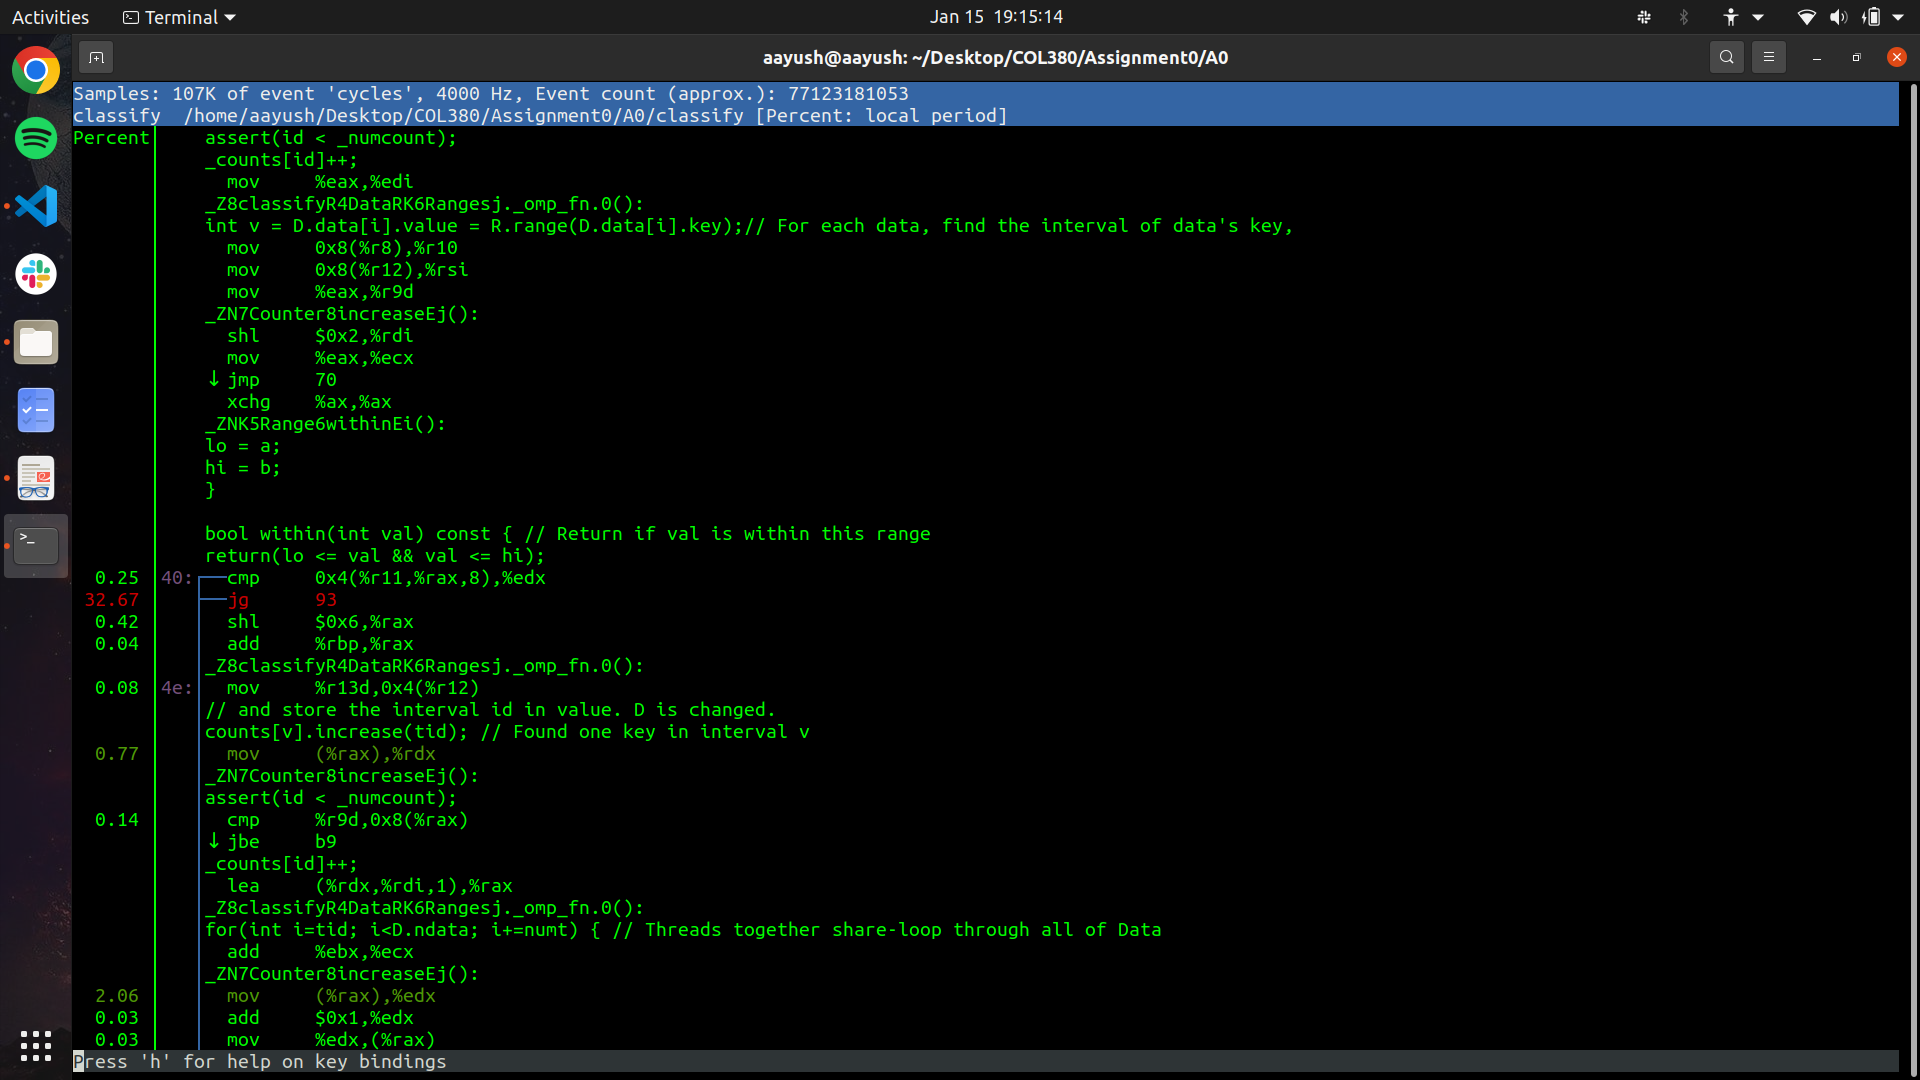
\includegraphics[width=1\textwidth]{images/2_5.png}
\end{figure}

\section{Hotspot Analysis}
\subsection{}
As shown in the screenshot above, the report is now showing source code along with assembly code. I have saved the perf data file with the appropriate name as mentioned in the assignment.

\subsection{}
Most amount of time is taken by the \texttt{jg 93} instruction. This is corresponding to the \texttt{within()} function.
\begin{figure}[H]
\centering  
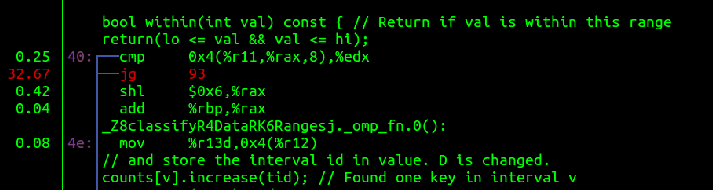
\includegraphics[width=1\textwidth]{images/hotspot.png}
\end{figure}

\subsection{}
The above mentioned instruction is probably a hotspot because the function is getting called a lot of times. For every data item we are traversing through the entire list of ranges. Morever the excessive time being taken at this point is because of poor caache utilization and false sharing. The above need to be resolved for making it more efficient.

\subsection{}
Yes, it is possible to optimize it further. One basic optimization possible in this case is that instead of using this as a function we can make it inline function. That is instead of doing another function call we can simply replace \texttt{within()} in the \texttt{Range::range()} function. This results in decent speedup because function calls are heavy. They require a lot of push and pop operations. Removing them will definitely make the code faster. The memory and cache related optimizations have been discussed in the further sections.

\subsection{}
To get the list of events which perf can record, run the command \texttt{perf list}. I ran the following command: \texttt{perf record -e branch-instructions,branch-misses,cache-misses,page-faults,cpu-cycles make run}
I have saved the perf.data file with the appropriate name as mentioned in the assignment.

\section{Memory Profiling}

\subsection{}
I ran \texttt{perf mem record make run} and saved the report with appropriate name as mentioned.

\subsection{}
Amongst the various hotspots, the following are the 2 major ones

\begin{enumerate}
    \item The first hotspot is in the first for loop of classify function.
\begin{figure}[H]
    \centering
    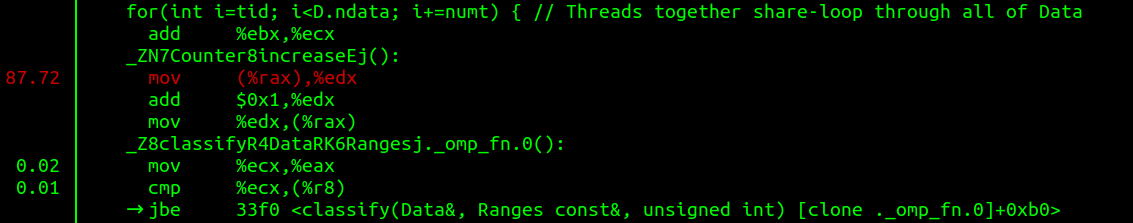
\includegraphics[width=1\textwidth]{images/hot2.png}
    \end{figure}
    \item Second is in the last for loop of the classify function.
\end{enumerate}

\begin{figure}[H]
\centering
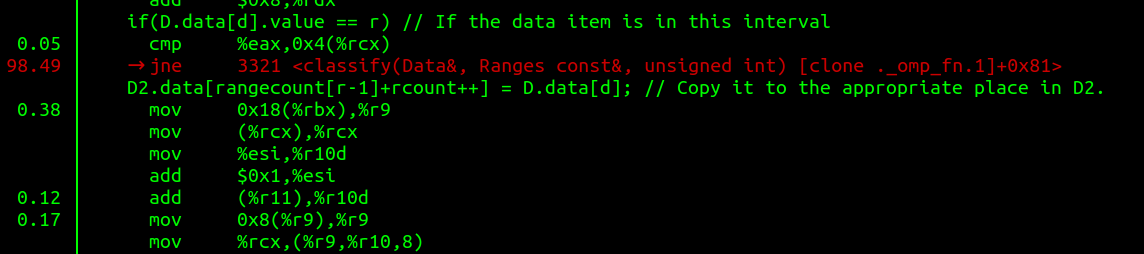
\includegraphics[width=1\textwidth]{images/hot1.png}
\end{figure}

\subsection{}
After reading the perf report I have analyzed different issues in the code. Their is false sharing happening and also instances of cache misses which can be avoided. The issues are:

\begin{enumerate}
    \item In the first for loop of the classify function and the last for loop of it, data is being accessed in a cyclic fashion in the threads. All the threads are trying to update the values in the same cache line. So every time, the cache line has to be updated in all of them. This is an instance of false sharing. We are not saving any time since we are updating the same cache line in all the threads. This can be resolved by dividing the data into contiguous chunks instead of cyclic chunks.
    \item Second issue is when we are updating the \texttt{count[v].increase(tid)}. Since the size of \texttt{counts[v]} array is small, the entire array gets stored in the cache. But when we are updating the \texttt{count[v].increase(tid)} in one thread, it needs to be updated in the other ones as well. Hence another instance of false sharing. This can be resolved using padding.
\end{enumerate}

\subsection{}

\begin{enumerate}
    \item As discussed in the above section about the instances of false sharing, I have tried to remove them by dividing the data into contiguous chunks instead of dividing the work in a cyclic manner. By allotting a big chunk to the thread we can avoid false sharing. ALl the adjacent array values belong to the same thread only and hence need not be updated in the other threads. This results in a significant speedup. I have implemented this change in both the first loop of classify function and the last loop of it. The time taken is 185.252ms which is a significant improvement over the initial time taken of 310.047ms.
    \item I have also removed the separate function call to \texttt{within()} and made it inline. This also reduced rhe run time to some extent since function calls are heavy, they require some significant amount of push and pop operations. 
\end{enumerate}
 
After doing these optimizations, I ran the \texttt{perf mem record make run} command and saved the report with appropriate name as mentioned. The hotspots earlier are not taking as much time as they were taking earlier. This is evident from the following screenshot.
\begin{enumerate}
    \item The first hotspot is in the first for loop of classify function. This is not taking any significant percent of time now.
    \begin{figure}[H]
        \centering
        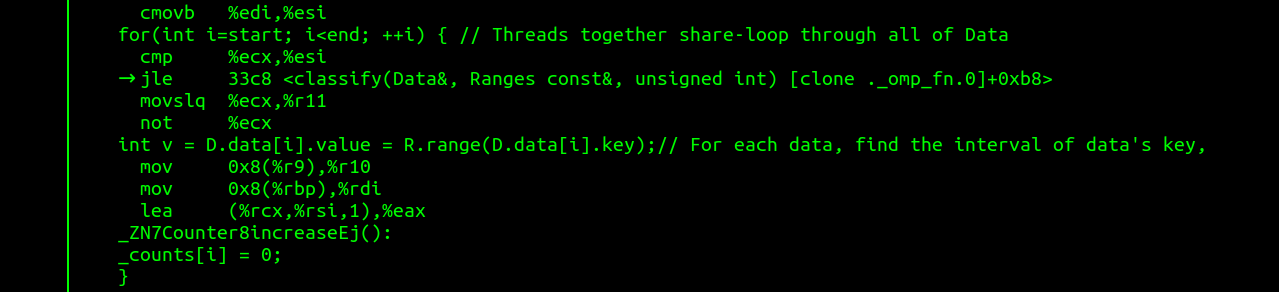
\includegraphics[width=1\textwidth]{images/upper_loop.png}
        \end{figure}
    \item Second is in the last for loop of the classify function. This is also not taking any significant percent of time now as compared to it was taking before.
    \begin{figure}[H]
    \centering
    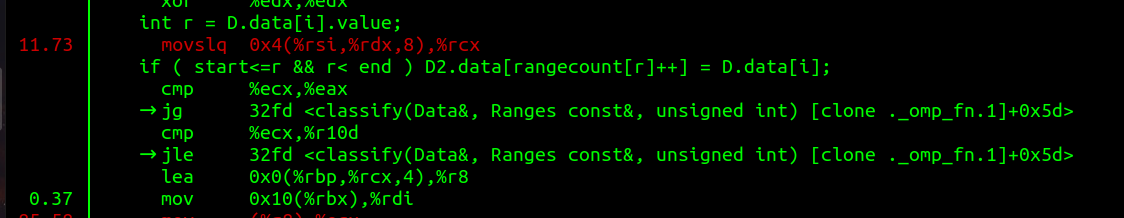
\includegraphics[width=1\textwidth]{images/lower_loop.png}
    \end{figure}
    
\end{enumerate}
Thus the optimizations have been successful in reducing the time taken by the hotspot of the code. The mem accesses have also decreased. All this has collectively resulted in decreased time taken by the code.




\subsection{}

\subsubsection{Runtime}

Initially the time taken was 310.047ms
\begin{figure}[H]
\centering
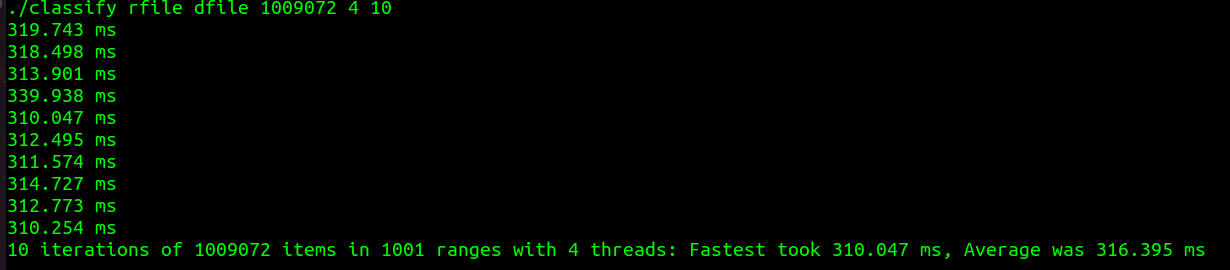
\includegraphics[width=1\textwidth]{images/316.png}
\end{figure}

After optimization time is 185.252ms 

\begin{figure}[H]
\centering
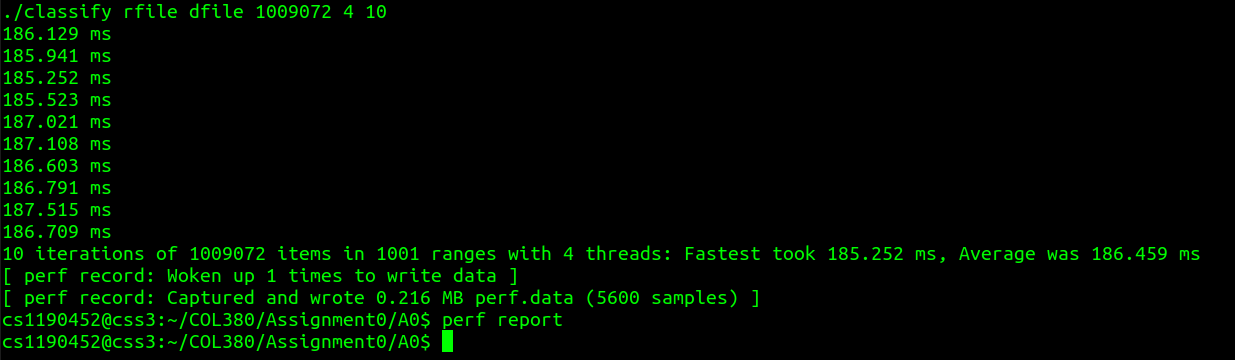
\includegraphics[width=1\textwidth]{images/186.png}
\end{figure}


Hence we can see after doing the optimizations there is a significant decrease in the time taken.

\subsubsection{Cache Misses}

Initially there were 8k events of cache misses 

\begin{figure}[H]
    \centering
    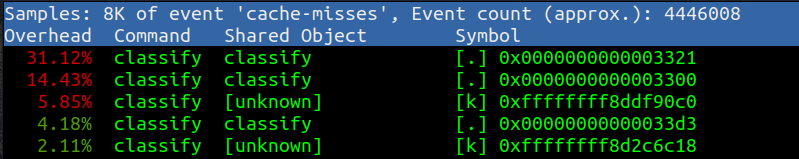
\includegraphics[width=1\textwidth]{images/8k.png}
    \end{figure}



Now there are only 5k events of cache misses after optimization

\begin{figure}[H]
    \centering
    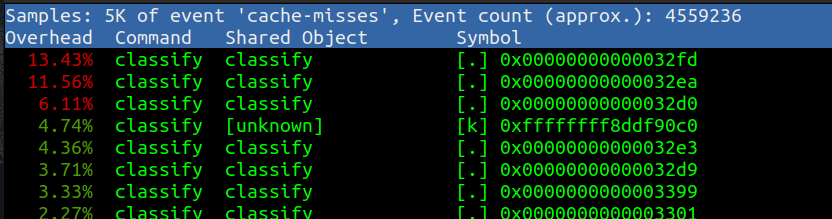
\includegraphics[width=1\textwidth]{images/5k.png}
    \end{figure}

Hence there have been a significant decrease in the number of cache misses, which has resulted in a significant decrease in the time taken.

\end{document}